% Note when we get to this section we can introduce temporal variation by stretching or shrinking our signals to augment our dataset to get more samples (and simulate potential an older adult).

\section{Selecting Cooking Tasks}
To employ some of the time-series classification methods discussed in Chapter \ref{chp:ts-classification}, a dataset of the proposed positional + IMU system is required. Chapter \ref{chp:lit-review}'s section on the traditional assessments of ADLs will serve as a basis for the selection of tasks to perform and collect data from. Of the assessments discussed, Table \ref{tab:cooking-task-summary} summarizes the assessments with cooking tasks mentioned in its procedure.

\begin{table}[ht]
    \small
    \centering
    \caption{Cooking tasks in the Assessment tools for the IADLs.}
    \label{tab:cooking-task-summary}
    \renewcommand{\arraystretch}{1.5}
    \begin{tabularx}{\textwidth}{>{\hsize=.8\hsize}X X }
        \hline
        \textbf{Tool} & \textbf{Tasks} \\
        \hline
        PASS & making soup with water/milk \\
        & making muffins in the oven \\
        & cutting up fruit \\
        Self-Assessment PD Disability Scale & making a cup of tea \\
        & inserting electrical plug \\
        & pouring milk from bottle \\
        & opening tins \\
        & washing \\
        Melbourne Low-vision ADL Index & preparing meals \\
        Lawton Instrumental ADL Scale & plans, prepares and serves adequate meals independently \\
        Frenchay Activities Index & preparing main meals \\
        Texas Functional Living Scale & Describe how to make peanut butter and jelly sandwich \\
        \hline
    \end{tabularx}
\end{table}

Of the assessments in Table \ref{tab:cooking-task-summary}, the cooking task(s) in the Melbourne Low-vision ADL Index, Lawton Instrumental ADL Scale, Frenchay Activities Index, and Self-Assessment PD Disability Scale are all questionnaires and as a result do not have concrete steps on how the task should be performed. Futhermore, the Melbourne Low-vision ADL Index, Lawnton Instrumental ADL Scale and the Frenchay Activities Index only have general requirements for the cooking task such as the ability to "prepare meals," and "plans, prepares and serves adequate meals independently." These general cooking tasks may be useful in the evaluation of ADL ability in a questionnaire format by requesting the older adult to holistically consider their ability to cook, but may not be the best candidates when looking for fine-grained actions to extract. 

The remaining 2 assessment tools, the Texas Functional Living Scale and Performance Assessment of Self-Care Skills (PASS), mention cooking task(s) that requires a clinician to evaluate. Upon closer inspection of the Texas Functional Living Scale, however, the individual is only required to describe the task and not actually perform it. The only candidate that has clear cooking tasks broken down into their fine-grained actions is the PASS and will be used as a reference for the experiment protocol and extraction of fine-grained tasks. 3 Cooking Scenarios are presented in the PASS: making soup with water/milk, making muffins in the oven, and cutting up fruit. The 3 cooking scenarios are shown in Figures \ref{fig:PASS-soup}-\ref{fig:PASS-muffin}.


\begin{figure}[ht]
    \centering
    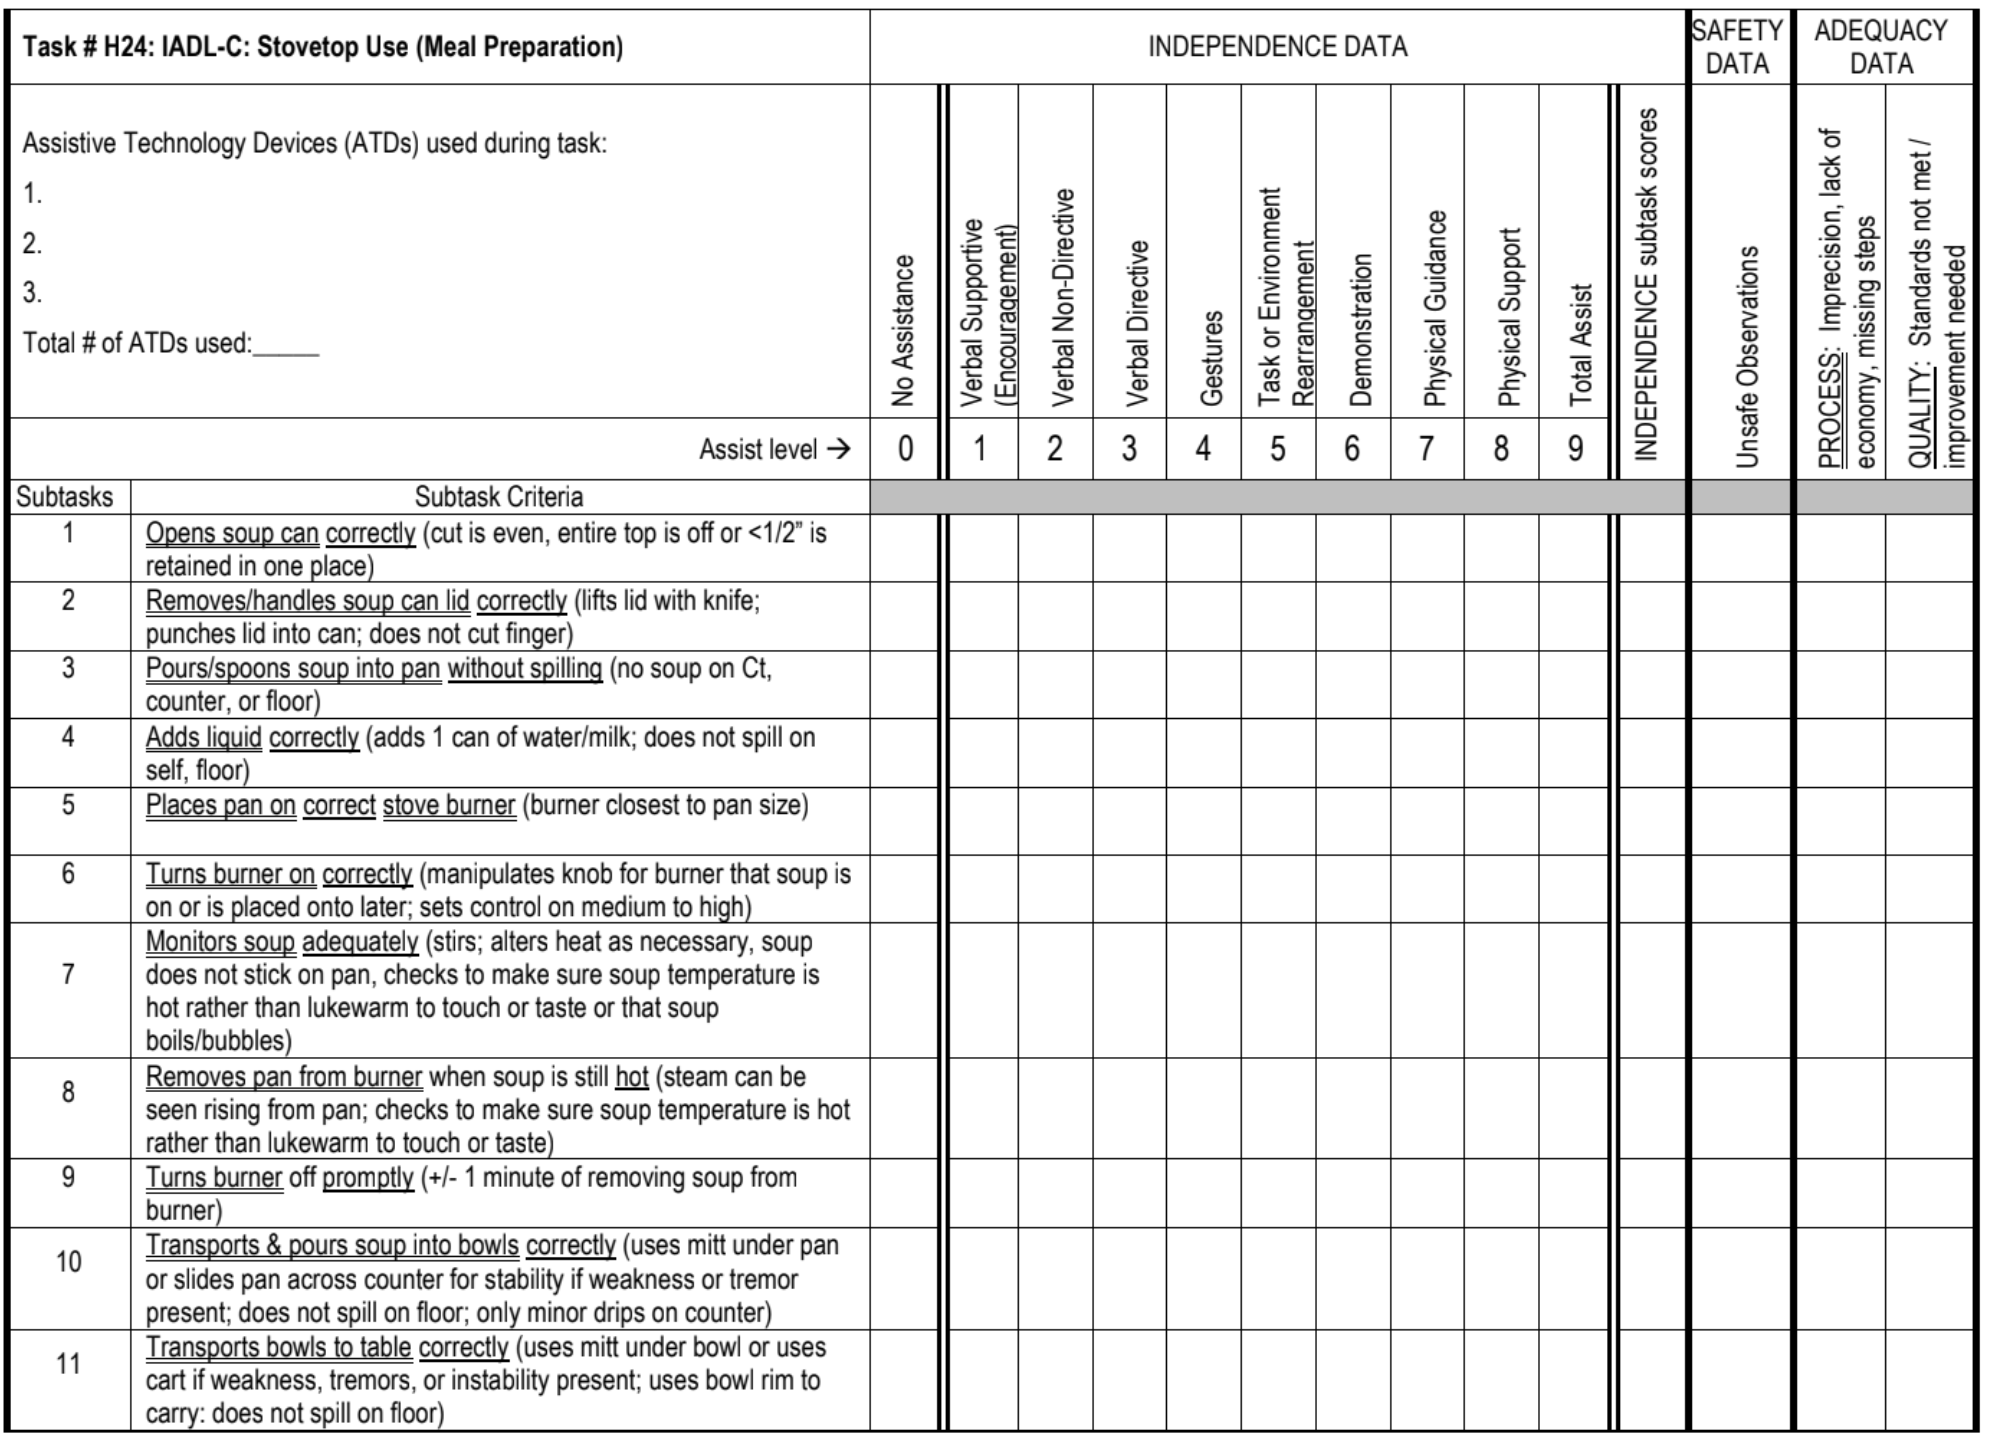
\includegraphics[width=0.8\textwidth]{pass-soup.png}
    \caption{PASS Soup Task \cite{rogers_performance_2014}}
    \label{fig:PASS-soup}
\end{figure}

\begin{figure}[ht]
    \centering
    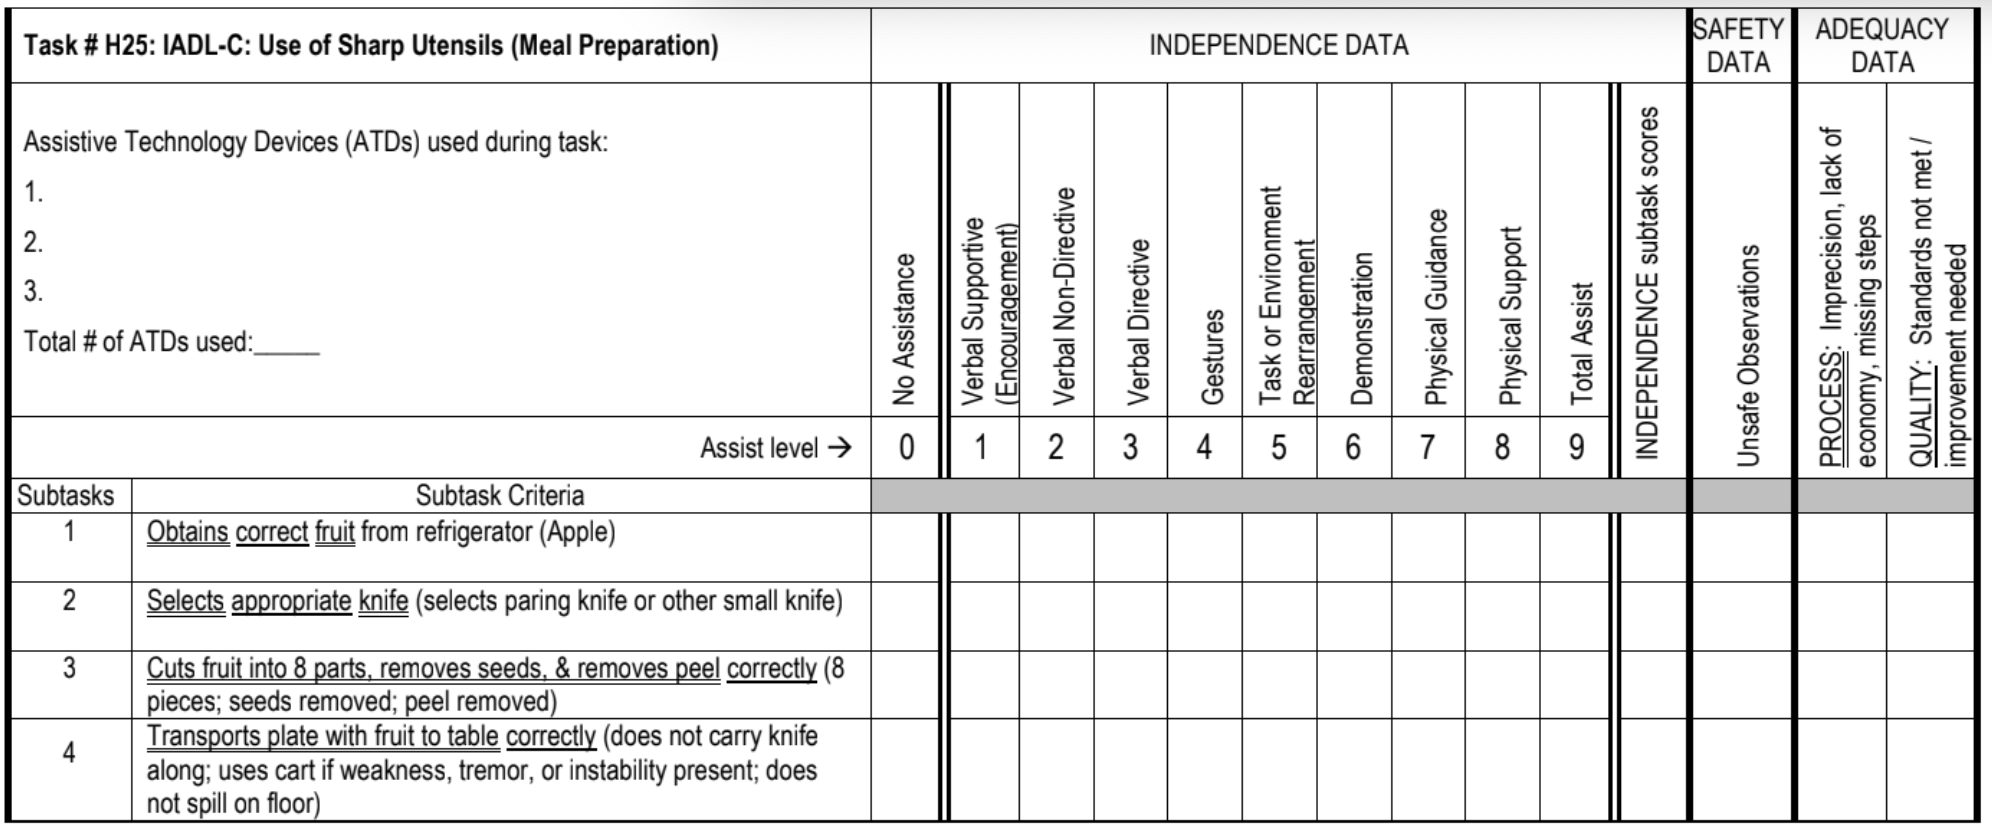
\includegraphics[width=0.8\textwidth]{pass-fruit.png}
    \caption{PASS Fruit Task \cite{rogers_performance_2014}}
    \label{fig:PASS-fruit}
\end{figure}

\begin{figure}[ht]
    \centering
    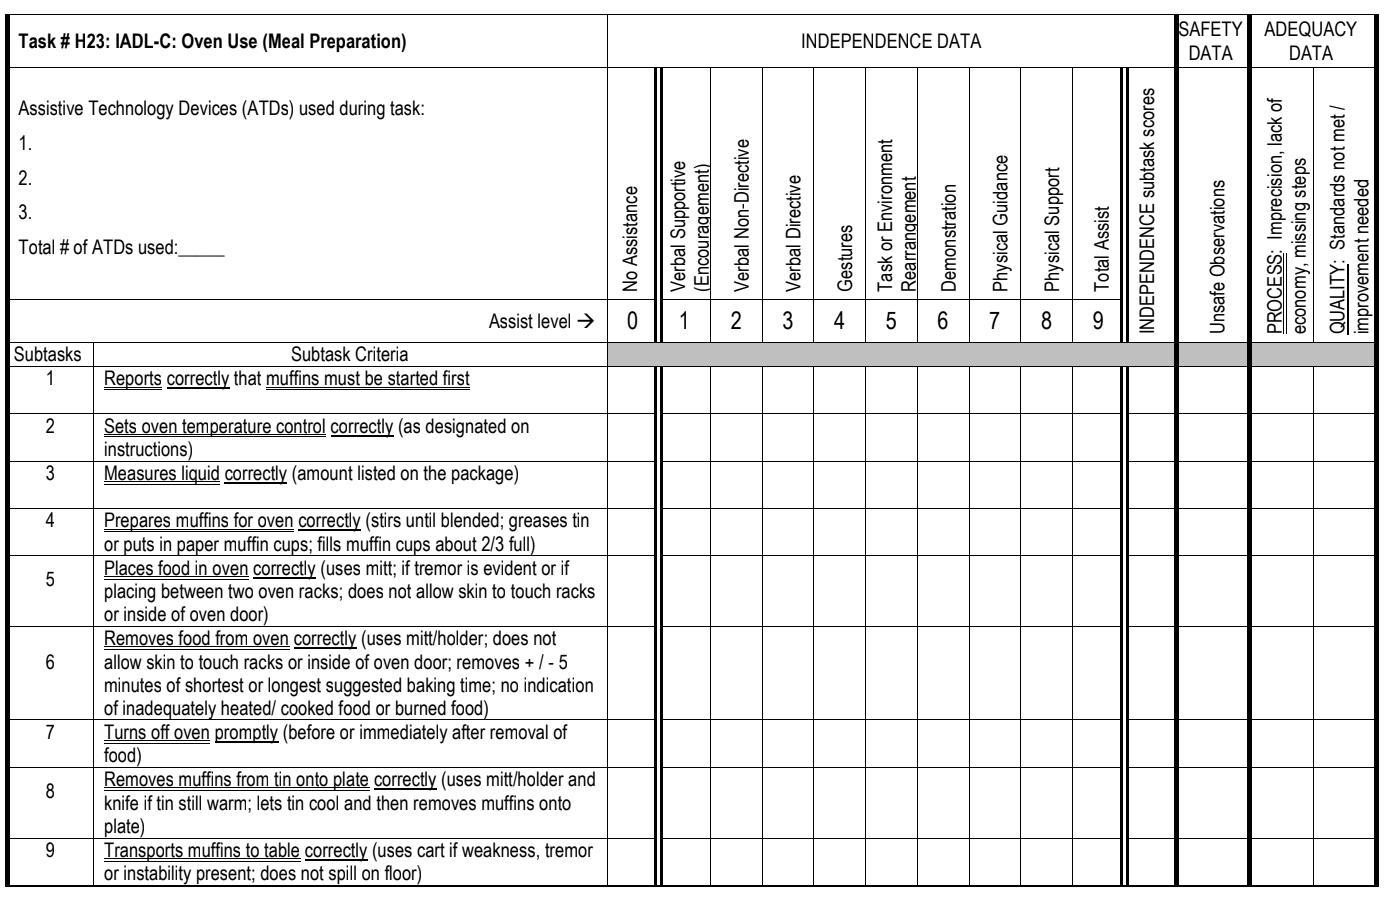
\includegraphics[width=0.8\textwidth]{pass-muffin.png}
    \caption{PASS Muffin Task \cite{rogers_performance_2014}}
    \label{fig:PASS-muffin}
\end{figure}

\clearpage
\section{Fine-grained Task Extraction}
The detail in which tasks can be broken down varies in literature. Human actions may be decomposed all the way into action primitives which is a body part + some motion (eg. right/left hand forward/backward) \cite{huszHumanActivityRecognition2007}. Fine-grained actions can be thought as being one level "coarser" than these action primitives and may combine action primitives to perform a small task (eg. cutting fruit, stir-frying, washing a fruit)  \cite{pan_fine-grained_2020}. A "coarser" level above fine-grained actions are coarse-grained actions and describe the activity that encompasses all of the fine-grained actions (eg. cooking, working). Although action primitives may be useful to consider when breaking down a task, the focus of the thesis is the evaluation of function and ability to perform tasks toward some goal. The detection of coarse-grained actions or activities have been successful in literature previously \cite{cook_learning_2010}, but these coarse-grained actions are too general and do not provide insight into the functional quality of the cooking task. Thus, the focus of the task extraction will be at the "fine-grained" level. 

For each cooking activity in the PASS, an experimental protocol will be developed based on the subtasks outlined in the task document. Although the PASS presents general steps to complete the task, there may sometimes be other actions, or "side-actions" involved in the task. For example, for the Cutting Fruit task in Figure \ref{fig:PASS-fruit}, obtaining the fruit from the refrigerator would require the individual to perform OPEN-FRIDGE, GRAB-FRIDGE, and CLOSE-FRIDGE. The experimental protocol will be more detailed with steps detailing the actions in the PASS as well as any side-actions that occur. Then, from the steps in the experimental protocol, the fine-grained actions can be extracted.

\section{Experimental Protocol}
This section will detail the experimental protocol for each of the 3 pass tasks. The steps presented in the original PASS document (Figures \ref{fig:PASS-fruit}-\ref{fig:PASS-muffin}) are used as reference and adapted to the environment where the experiments will take place: the Independent Living Suite.

\subsection{Initial Setup}
The initial setup prior to conducting the experiments involved the following steps:

\begin{enumerate}
    \item Referencing the 9H configuration the resulted in the best accuracy and repeatability determined in Chapter \ref{chp:sys-tuning}, the anchors are set up in the locations indicated by Figure \ref{fig:anchorplacement}.
    \item Based on the documentation for the Pozyx \cite{pozyx_configuration_nodate}, the settings for the fastest possible sample rate (16 Hz) without a large effect on the communication range was a bitrate of 850 kbit/s and a preamble length of 128. Both the anchors and the tags were set to communicate at these settings.
    \item Setup a camera with a countdown timer so that segments of the data can be manually labelled at a later time.
    \item Wear the Pozyx tag on the dominant hand.
\end{enumerate}

\subsection{Protocol: Cutting Fruit}
Based on Figure \ref{fig:PASS-fruit}, this task involves getting a piece of fruit from the refrigerator, choosing a knife, peeling the fruit, cutting it into 8 pieces, plating and serving it. The detailed steps for the protocol are shown in Table \ref{tab:protocol-cutting-fruit} with the fruit being an apple.

\small
\centering
\renewcommand{\arraystretch}{1.5}
\clearpage
\begin{xltabular}{\textwidth}{>{\hsize=.15\hsize}X X >{\hsize=.4\hsize}X}
\caption{Protocol for the PASS cutting fruit task. Note that Quiet Standing (QS) refers to the position where the participant has their hands on the side of their thighs, being as still as possible.} \label{tab:protocol-cutting-fruit} \\

% First Header
\hline \textbf{Step} & \textbf{Details} & \textbf{Fine-Grained Action} \\ \hline 
\endfirsthead

% Subsequent headers.
\multicolumn{3}{c}{\tablename\ \thetable{} -- continued from previous page} \\
\hline \textbf{Step} & \textbf{Details} & \textbf{Fine-Grained Action} \\ \hline 
\endhead

% Footers
\hline \multicolumn{3}{r}{\textit{Continued on next page}} \\ \hline
\endfoot

% Last Footer
\hline
\endlastfoot

% The Table
    1 & Start the video with the countdown and just as the countdown finishes start data collection script & \\ 
    2 & Move to the position in front of the refrigerator and stand in a Quiet Standing (QS) position for 2-3 seconds. Quickly raise and lower the hand with the sensor (for sensor and video time synchronization) and return to QS & \\ 
    3 & Stay in QS for 5 seconds & QS \\
    4 & Walk to the sink & \\
    5 & Open the faucet and wash hands for 10 seconds, close the faucet & WASH \\
    6 & Walk to the position in front of the oven (where the drying towel is) &  \\
    7 & Dry hands & DRY \\
    8 & Walk to the position in front of the refrigerator & \\
    9 & Open the refrigerator with the dominant hand & OPEN-FRIDGE \\
    10 & Reach into the fridge and grab an apple with the dominant hand & GRAB-FRIDGE \\
    11 & Close the fridge with the dominant hand & CLOSE-FRIDGE \\
    12 & Place the apple on the kitchen counter & \\
    13 & Walk to where the cutting board is & \\
    14 & Grab the cutting board & GRAB-BOARD \\
    15 & Walk to the kitchen counter & \\
    16 & Place the cutting board on the kitchen counter (beside the apple) & \\
    17 & Move to the position in front of the drawer containing the knife & \\
    18 & Open the drawer with the knife with the dominant hand & OPEN-CUTLERY \\
    19 & Grab the parring knife with the dominant hand & GRAB-CUTLERY \\
    20 & Close the drawer with the dominant hand & CLOSE-CUTLERY \\
    21 & Place the knife on the counter & \\
    22 & Grab the apple and move to the position in front of the sink & \\
    23 & Wash the apple & WASH \\
    24 & Move back to the position in front of the counter &  \\
    25 & Peel the apple using the parring knife & PEEL \\
    26 & Cut the apple into 8ths using the chopping board & CUT \\
    27 & Move to the position in front of the tableware cabinet & \\
    28 & Open the tableware cabinet door & OPEN-TABLEWARE \\
    29 & Grab a plate and place it on the kitchen counter & GRAB-TABLEWARE \\
    30 & Close the tableware cabinet & CLOSE-TABLEWARE \\
    31 & Move to the position in front of the kitchen counter & \\
    32 & Transfer the apple slices from the cutting board to the plate & PLATING \\
    33 & Grab the plate with the apples and bring place it on the dining table & SERVE \\
    34 & Return to the position in front of the refrigerator and stand in QS for 5 seconds & QS \\
    \hline
\end{xltabular}

\clearpage
\subsection{Protocol: Making Soup}
